\begin{center}
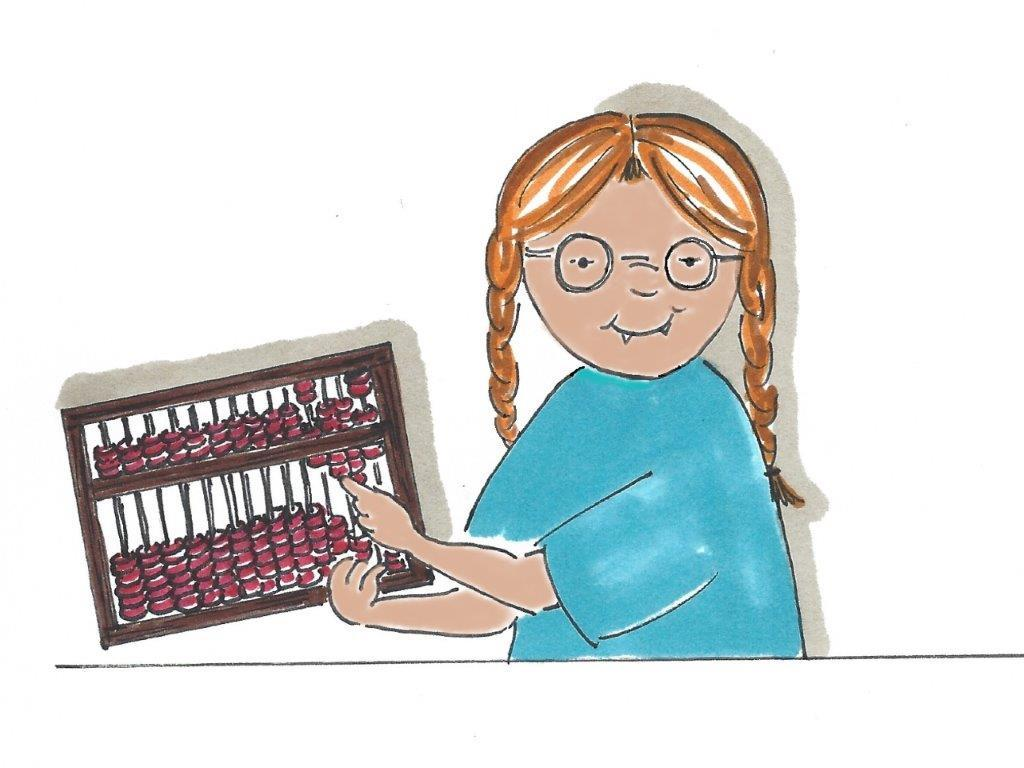
\includegraphics[width=0.6\textwidth]{content/3/chapter5/images/15.png}\\
Cippi在研究算盘
\end{center}

有符号整数和无符号整数的比较,有时导致意外行为和错误的原因。C++20添加了新的类型安全的比较函数std::cmp\_*,相应的错误就能完全避免了。此外,C++20还包含了一些数学常数,比如e、π或φ,使用函数std::midpoint和std::lerp,你可以计算两个数的中点或它们的线性插值。新的位操作可以访问和修改单个位或位序列。

\subsubsubsection{5.4.1\hspace{0.2cm}整型数的安全比较}

比较有符号整数和无符号整数时,可能得不到预期的结果。C++20添加了六个std::cmp\_*函数,使得比较更加安全。为了更好的了解添加整数安全比较意义,这里先从不安全比较开始说起。

\begin{tcolorbox}[breakable,enhanced jigsaw,colback=blue!5!white,colframe=blue!75!black,title={整数与整型}]
	
术语integral(整数)和integer(整型)是C++中的同义词。这是基本类型标准的表述:“类型bool, char, char8\_t, char16\_t, char32\_t, wchar\_t,以及有符号整型和无符号整型统称为整数类型。整数是某一种具体的整型”。本书里,我更喜欢用整型这个词。
	
\end{tcolorbox}

\hspace*{\fill} \\ %插入空行
\noindent
\textbf{5.4.1.1\hspace{0.2cm}不安全的比较}

当然,下面这段代码的名称为unsafcompare.cpp,命名成这样是有原因的。

\begin{lstlisting}[style=styleCXX]
// unsafeComparison.cpp

#include <iostream>

int main() {
	
	std::cout << '\n';
	
	std::cout << std::boolalpha;
	
	int x = -3;
	unsigned int y = 7;
	
	std::cout << "-3 < 7: " << (x < y) << '\n';
	std::cout << "-3 <= 7: " << (x <= y) << '\n';
	std::cout << "-3 > 7: " << (x > y) << '\n';
	std::cout << "-3 => 7: " << (x >= y) << '\n';
	
	std::cout << '\n';

}
\end{lstlisting}

当执行时,输出可能不符合期望。

\begin{tcblisting}{commandshell={}}
-3 < 7: false
-3 <= 7: false
-3 > 7: true
-3 => 7: true
\end{tcblisting}

\begin{center}
不安全的比较结果令人惊讶
\end{center}

看到程序的输出时,会发现-3比7大。我想你大概知道为什么会这样。我比较了有符号的x(第11行)和无符号的y(第12行)。这背后发生了什么?下面的代码会告诉我们答案。

\hspace*{\fill} \\ %插入空行
\noindent
\textbf{解决不安全的整数比较}
\begin{lstlisting}[style=styleCXX]
// unsafeComparison2.cpp

int main() {
	int x = -3;
	unsigned int y = 7;
	
	bool val = x < y;
	static_assert(static_cast<unsigned int>(-3) == 4'294'967'293);
}
\end{lstlisting}

本例中,主要关注小于操作符。\href{https://cppinsights.io/s/62732a01}{C++ Insights}输出如下:

\begin{lstlisting}[style=styleCXX]
int main()
{
	int x = -3;
	unsigned int y = 7;
	bool val = static_cast<unsigned int>(x) < y;
	/* PASSED: static_assert(static_cast<long>(static_cast<unsigned int>(-3)) == 4294967293L); */
	return 0;
}
\end{lstlisting}
\begin{center}
分析不安全的比较
\end{center}

事情是这样的:

\begin{itemize}
\item 
编译器将表达式x < y(第7行)转换为static\_cast<unsigned int>(x) < y。特别地,有符号x转换为无符号int类型。

\item 
因为这个转换,-3变成了4'294'967'293。

\item 
4'294'967'293等于$ 2^{32} $加−3

\item 
32是C++ Insights中无符号整型的位宽。
\end{itemize}

由于C++20的出现,现在可以安全地对整数进行比较了。

\hspace*{\fill} \\ %插入空行
\noindent
\textbf{5.4.1.2\hspace{0.2cm}安全的整数比较}

C++20支持6个整数比较函数:

\begin{center}
六种安全比较函数
\end{center}

\begin{table}[H]
\centering
\begin{tabular}{ll}
\textbf{比较函数} & \textbf{描述} \\ \hline
std::cmp\_equal           & ==               \\
std::cmp\_not\_equal      & !=               \\
std::cmp\_less            & \textless{}      \\
std::cmp\_less\_equal     & \textless{}=     \\
std::cmp\_greater         & \textgreater{}   \\
std::cmp\_greater\_equal  & \textgreater{}= 
\end{tabular}
\end{table}

由于这个六个比较函数的出现,现在可以轻松地将之前的程序unsafecomparis.cpp改写为safecomparis.cpp。新的比较函数需要头文件<utility>。

\begin{lstlisting}[style=styleCXX]
// safeComparison.cpp

#include <iostream>
#include <utility>

int main() {
	
	std::cout << '\n';
	
	std::cout << std::boolalpha;
	
	int x = -3;
	unsigned int y = 7;
	
	std::cout << "-3 == 7: " << std::cmp_equal(x, y) << '\n';
	std::cout << "-3 != 7: " << std::cmp_not_equal(x, y) << '\n';
	std::cout << "-3 < 7: " << std::cmp_less(x, y) << '\n';
	std::cout << "-3 <= 7: " << std::cmp_less_equal(x, y) << '\n';
	std::cout << "-3 > 7: " << std::cmp_greater(x, y) << '\n';
	std::cout << "-3 => 7: " << std::cmp_greater_equal(x, y) << '\n';
	
	std::cout << '\n';
	
}
\end{lstlisting}

另外,这里使用了等号和不等号运算符。

\begin{tcblisting}{commandshell={}}
-3 == 7: false
-3 != 7: true
-3 < 7: true
-3 <= 7: true
-3 > 7: false
-3 => 7: false
\end{tcblisting}

使用非整数(如double)调用安全比较函数会导致编译时错误。

\hspace*{\fill} \\ %插入空行
\noindent
\textbf{尝试安全比较uint和double}
\begin{lstlisting}[style=styleCXX]
// safeComparison2.cpp

#include <iostream>
#include <utility>

int main() {
	
	double x = -3.5;
	unsigned int y = 7;
	
	std::cout << "-3.5 < 7: " << std::cmp_less(x, y); // ERROR
	
}
\end{lstlisting}

另外,还是可以用经典的方法比较double型和unsigned型的数值。classicalcompare.cpp就使用了double类型和unsigned int类型的经典比较方式。

\hspace*{\fill} \\ %插入空行
\noindent
\textbf{uint和double的经典比较方式}
\begin{lstlisting}[style=styleCXX]
// classicalComparison.cpp

int main() {
	
	double x = -3.5;
	unsigned int y = 7;
	
	auto res = x < y; // true
	
}
\end{lstlisting}

没毛病!unsigned int将\href{https://en.cppreference.com/w/cpp/language/implicit_conversion}{升格为浮点},再提升为double。\href{https://cppinsights.io/s/44216566}{C++ Insights}展示了实际发生了什么:

\begin{center}
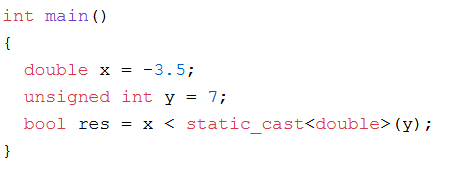
\includegraphics[width=0.6\textwidth]{content/3/chapter5/images/1-5.png}\\
浮点提升为double
\end{center}

\subsubsubsection{5.4.2\hspace{0.2cm}数学常数}

首先,数学常数要求头文件<numbers>和命名空间std::numbers,下表提供了一个概述。

\begin{table}[H]
\centering
\begin{tabular}{ll}
Mathematical Constant     & Description               \\ \hline
std::numbers::e           & $e$                       \\
std::numbers::log2e       & $log_{2}e$                \\
std::numbers::log10e      & $log_{10}e$               \\
std::unmbers::pi          & $\pi$                     \\
std::unmbers::inv\_pi     & $\frac{1}{\pi}$           \\
std::numbers::inv\_sqrtpi & $\frac{1}{\sqrt{\pi}}$    \\
std::numbers::ln2         & ln2                       \\
std::numbers::ln10        & ln10                      \\
std::numbers::sqrt2       & $\sqrt{2}$                \\
std::numbers::sqrt3       & $\sqrt{3}$                \\
std::numbers::inv\_sqrt3  & $\frac{1}{\sqrt{3}}$      \\
std::numbers::egamma      & \href{https://en.wikipedia.org/wiki/Euler%E2%80%93Mascheroni_constant}{欧拉常数(Euler-Mascheroni常数)} \\
std::numbers::phi         & $\phi$                   
\end{tabular}
\end{table}

mathematicConstants.cpp使用了一些数学常数。

\begin{lstlisting}[style=styleCXX]
// mathematicConstants.cpp

#include <iomanip>
#include <iostream>
#include <numbers>

int main() {
	std::cout << '\n';
	
	std::cout<< std::setprecision(10);
	
	std::cout << "std::numbers::e: " << std::numbers::e << '\n';
	std::cout << "std::numbers::log2e: " << std::numbers::log2e << '\n';
	std::cout << "std::numbers::log10e: " << std::numbers::log10e << '\n';
	std::cout << "std::numbers::pi: " << std::numbers::pi << '\n';
	std::cout << "std::numbers::inv_pi: " << std::numbers::inv_pi << '\n';
	std::cout << "std::numbers::inv_sqrtpi: " << std::numbers::inv_sqrtpi << '\n';
	std::cout << "std::numbers::ln2: " << std::numbers::ln2 << '\n';
	std::cout << "std::numbers::sqrt2: " << std::numbers::sqrt2 << '\n';
	std::cout << "std::numbers::sqrt3: " << std::numbers::sqrt3 << '\n';
	std::cout << "std::numbers::inv_sqrt3: " << std::numbers::inv_sqrt3 << '\n';
	std::cout << "std::numbers::egamma: " << std::numbers::egamma << '\n';
	std::cout << "std::numbers::phi: " << std::numbers::phi << '\n';
	
	std::cout << '\n';
}
\end{lstlisting}

下面是使用MSVC编译器生成程序的输出。

\begin{tcblisting}{commandshell={}}
std::numbers::e: 2.718281828
std::numbers::log2e: 1.442695041
std::numbers::log10e: 0.4342944819
std::numbers::pi: 3.141592654
std::numbers::inv_pi: 0.3183098862
std::numbers::inv_sqrtpi: 0.5641895835
std::numbers::ln2: 0.6931471806
std::numbers::sqrt2: 1.414213562
std::numbers::sqrt3: 1.732050808
std::numbers::inv_sqrt3: 0.5773502692
std::numbers::egamma: 0.5772156649
std::numbers::phi: 1.618033989
\end{tcblisting}

\begin{center}
使用所有的数学常数
\end{center}

数学常数可用于float、double和long double。默认情况下,使用double。但也可以指定float (std::numbers::pi\_v<float>)或long double (std::numbers::pi\_v<long double>)。

\subsubsubsection{5.4.3\hspace{0.2cm}中间值与线性插值}

\begin{itemize}
\item 
std::midpoint(a, b):计算整数、浮点数或指针的中点(a + (b - a) / 2)。若a和b是指针,则必须指向同一个数组对象。该函数需要头文件<numeric>。

\item 
std::lerp(a, b, t):计算线性插值(a + t(b - a))。当t在范围[0,1]之外时,则计算线性外推。函数需要头文件<cmath>。
\end{itemize}

midpointLerp.cpp使用这两个函数。

\hspace*{\fill} \\ %插入空行
\noindent
\textbf{计算中点和数字的线性插值}
\begin{lstlisting}[style=styleCXX]
// midpointLerp.cpp

#include <cmath>
#include <numeric>
#include <iostream>

int main() {
	
	std::cout << '\n';
	
	std::cout << "std::midpoint(10, 20): " << std::midpoint(10, 20) << '\n';
	
	std::cout << '\n';
	
	for (auto v: {0.0, 0.1, 0.2, 0.3, 0.4, 0.5, 0.6, 0.7, 0.8, 0.9, 1.0}) {
		std::cout << "std::lerp(10, 20, " << v << "): " << std::lerp(10, 20, v)
				  << '\n';
	}
	
	std::cout << '\n';
	
}
\end{lstlisting}

程序及其输出就没什么好说的了:

\begin{tcblisting}{commandshell={}}
std::midpoint(10, 20): 15

std::midpoint(10, 20, 0): 10
std::midpoint(10, 20, 0.1): 11
std::midpoint(10, 20, 0.2): 12
std::midpoint(10, 20, 0.3): 13
std::midpoint(10, 20, 0.4): 14
std::midpoint(10, 20, 0.5): 15
std::midpoint(10, 20, 0.6): 16
std::midpoint(10, 20, 0.7): 17
std::midpoint(10, 20, 0.8): 18
std::midpoint(10, 20, 0.9): 19
std::midpoint(10, 20, 1): 20
\end{tcblisting}

\subsubsubsection{5.4.4\hspace{0.2cm}位操作}

头文件<bit>声明了访问和操作单个位或位序列的函数。

\hspace*{\fill} \\ %插入空行
\noindent
\textbf{5.4.4.1\hspace{0.2cm}std::endian}

新类型std::endian,可以获得标量类型的字节序。端序可以是大端序或小端序。大端表示高位字节在最左边,小端表示低位字节在最左边。标量类型可以是算术类型、枚举、指针、成员指针或std::nullptr\_t。

endian类提供了所有标量类型的端序:

\hspace*{\fill} \\ %插入空行
\noindent
\textbf{枚举类endian}
\begin{lstlisting}[style=styleCXX]
enum class endian
{
	little = /*implementation-defined*/,
	big = /*implementation-defined*/,
	native = /*implementation-defined*/
};
\end{lstlisting}

\begin{itemize}
\item 
若所有标量类型都是小端,则std::endian::native等于std::endian::little。

\item 
若所有标量类型都是大端,则std::endian::native等于std::endian::big。
\end{itemize}

即使是极端情况也支持:

\begin{itemize}
\item 
若所有的标量类型都具有sizeof 1,端序就不重要了,枚举数std::endian::little、std::endian::big和std::endian::native的值是相同的。

\item 
若平台使用混合字节序,std::endian::native既不等于std::endian::big,也不等于std::endian::little。
\end{itemize}

当在x86架构上执行下面的getEndianness.cpp时,我得到的结果是little-endian。

\begin{lstlisting}[style=styleCXX]
// getEndianness.cpp

#include <bit>
#include <iostream>

int main() {
	
	if constexpr (std::endian::native == std::endian::big) {
		std::cout << "big-endian" << '\n';
	}
	else if constexpr (std::endian::native == std::endian::little) {
		std::cout << "little-endian" << '\n'; // little-endian
	}

}
\end{lstlisting}

constexpr if使编译器能够有条件地编译源代码。所以,编译依赖于架构的字节序。

\hspace*{\fill} \\ %插入空行
\noindent
\textbf{5.4.4.2\hspace{0.2cm}访问,位操作,位序列}

下表概述了所有函数,可以在头文件<bit>中找到相应的函数。

\begin{center}
位操作
\end{center}

\begin{table}[H]
\centering
\begin{tabular}{ll}
\textbf{函数}     & \textbf{描述}                                                             \\ \hline
std::bit\_cast        & 重新解释对象的表示                                           \\
std::has\_single\_bit & 检查数字是否为2的次幂                                             \\
std::bit\_ceil        & 求不小于给定值的2的最小整数次幂 \\
std::bit\_floor       & 求不大于给定值的2的最大整数次幂  \\
std::bit\_width       & 找到表示给定值的最小位数                   \\
std::rotl             & 计算按位向左移                                               \\
std::rotr             & 计算按位向右移                                               \\
std::countl\_zero     & 从最高位开始,计数连续0的个数      \\
std::countl\_one      & 从最高位开始,计算连续1的个数      \\
std::countr\_zero     & 从最低位开始,计数连续0的个数    \\
std::countr\_one      & 从最低有效位,计算连续1的个数     \\
std::popcount         & 统计无符号整数中位值为1的个数                                  
\end{tabular}
\end{table}

除std::bit\_cast外,所有函数都要求是无符号整数类型(unsigned char、unsigned short、unsigned int、unsigned long或unsigned long)。

bit.cpp展示了如何使用这些函数。

\hspace*{\fill} \\ %插入空行
\noindent
\textbf{位操作}
\begin{lstlisting}[style=styleCXX]
// bit.cpp

#include <bit>
#include <bitset>
#include <iostream>

int main() {
	
	std::uint8_t num= 0b00110010;
	
	std::cout << std::boolalpha;
	
	std::cout << "std::has_single_bit(0b00110010): " << std::has_single_bit(num)
	          << '\n';
	          
	std::cout << "std::bit_ceil(0b00110010): " << std::bitset<8>(std::bit_ceil(num))
	          << '\n';          
	std::cout << "std::bit_floor(0b00110010): "
	          << std::bitset<8>(std::bit_floor(num)) << '\n';
	
	std::cout << "std::bit_width(5u): " << std::bit_width(5u) << '\n';
	
	std::cout << "std::rotl(0b00110010, 2): " << std::bitset<8>(std::rotl(num, 2))
	          << '\n';
	
	std::cout << "std::rotr(0b00110010, 2): " << std::bitset<8>(std::rotr(num, 2))
	          << '\n';
	          
	std::cout << "std::countl_zero(0b00110010): " << std::countl_zero(num) << '\n';
	std::cout << "std::countl_one(0b00110010): " << std::countl_one(num) << '\n';
	std::cout << "std::countr_zero(0b00110010): " << std::countr_zero(num) << '\n';
	std::cout << "std::countr_one(0b00110010): " << std::countr_one(num) << '\n';
	std::cout << "std::popcount(0b00110010): " << std::popcount(num) << '\n';
}
\end{lstlisting}

下面是程序的输出。

\begin{tcblisting}{commandshell={}}
std::has_single_bit(0b00110010): false
std::bit_ceil(0b00110010): 01000000
std::bit_floor(0b00110010): 00100000
std::bit_width(5u): 3
std::rotl(0b00110010, 2): 11001000
std::rotr(0b00110010, 2): 10001100
std::countl_zero(0b00110010): 2
std::countl_one(0b00110010): 0
std::countr_zero(0b00110010): 1
std::countr_one(0b00110010): 0
std::popcount(0b00110010): 3
\end{tcblisting}

下面的程序显示了,将std::bit\_floor, std::bit\_ceil, std::bit\_width和std::bit\_popcount用于数字2到7的效果。

\begin{lstlisting}[style=styleCXX]
// bitFloorCeil.cpp

#include <bit>
#include <bitset>
#include <iostream>

int main() {
	
	std::cout << '\n';
	
	std::cout << std::boolalpha;
	
	for (auto i = 2u; i < 8u; ++i) {
		std::cout << "bit_floor(" << std::bitset<8>(i) << ") = "
		          << std::bit_floor(i) << '\n';
		
		std::cout << "bit_ceil(" << std::bitset<8>(i) << ") = "
		          << std::bit_ceil(i) << '\n';
		
		std::cout << "bit_width(" << std::bitset<8>(i) << ") = "
		          << std::bit_width(i) << '\n';
		
		std::cout << "popcount(" << std::bitset<8>(i) << ") = "
		          << std::popcount(i) << '\n';
		
		std::cout << '\n';
	}

	std::cout << '\n';
}
\end{lstlisting}

\begin{tcblisting}{commandshell={}}
bit_floor(00000010) = 2
bit_ceil(00000010) = 2
bit_width(00000010) = 2
popcount(00000010) = 1

bit_floor(00000011) = 2
bit_ceil(00000011) = 4
bit_width(00000011) = 2
popcount(00000011) = 2

bit_floor(00000100) = 4
bit_ceil(00000100) = 4
bit_width(00000100) = 3
popcount(00000100) = 1

bit_floor(00000101) = 4
bit_ceil(00000101) = 8
bit_width(00000101) = 3
popcount(00000101) = 2

bit_floor(00000110) = 4
bit_ceil(00000110) = 8
bit_width(00000110) = 3
popcount(00000110) = 2

bit_floor(00000111) = 4
bit_ceil(00000111) = 8
bit_width(00000111) = 3
popcount(00000111) = 3
\end{tcblisting}

\begin{center}
对一些数字使用std::bit\_floor, std::bit\_ceil, std::bit\_width和std::popcount
\end{center}

\begin{tcolorbox}[breakable,enhanced jigsaw,colback=mygreen!5!white,colframe=mygreen!75!black,title={总结}]
	
\begin{itemize}
\item 
C++20中的cmp\_*函数支持安全的整数比较,其可以检测有符号整数和无符号整数的比较。在不安全比较的情况下,编译会失败。

\item 
并且,定义了许多数学常数,如$e$、$log_2e$或$\pi$。

\item 
C++20提供了计算两个值的中点或线性插值的工具函数。

\item 
有新函数可以访问和操作位或位序列。
\end{itemize}
	
\end{tcolorbox}
\newpage